
% Complete documentation on the extended LaTeX markup used for Insight
% documentation is available in ``Documenting Insight'', which is part
% of the standard documentation for Insight.  It may be found online
% at:
%
%     http://www.itk.org/

\documentclass{InsightArticle}

\usepackage[dvips]{graphicx}
\usepackage{xspace}
\usepackage{dsfont}
%%%%%%%%%%%%%%%%%%%%%%%%%%%%%%%%%%%%%%%%%%%%%%%%%%%%%%%%%%%%%%%%%%
%
%  hyperref should be the last package to be loaded.
%
%%%%%%%%%%%%%%%%%%%%%%%%%%%%%%%%%%%%%%%%%%%%%%%%%%%%%%%%%%%%%%%%%%
\usepackage[dvips,
bookmarks,
bookmarksopen,
backref,
colorlinks,linkcolor={blue},citecolor={blue},urlcolor={blue},
]{hyperref}


%  This is a template for Papers to the Insight Journal. 
%  It is comparable to a technical report format.

% The title should be descriptive enough for people to be able to find
% the relevant document. 
\title{Statismo - A framework for PCA based statistical models.}

% 
% NOTE: This is the last number of the "handle" URL that 
% The Insight Journal assigns to your paper as part of the
% submission process. Please replace the number "1338" with
% the actual handle number that you get assigned.
%
\newcommand{\IJhandlerIDnumber}{1338}
\newcommand{\statismo}{\emph{statismo}\xspace}
\newcommand{\Statismo}{\emph{Statismo}\xspace}
\def\R{\mathds{R}} %reelle Zahlen

% Increment the release number whenever significant changes are made.
% The author and/or editor can define 'significant' however they like.
\release{0.80}

% At minimum, give your name and an email address.  You can include a
% snail-mail address if you like.
\author{Marcel L\"uthi$^{1}$, R{\'e}mi Blanc$^{2}$, Thomas Albrecht$^{1}$, Tobias Gass$^{3}$, Orcun Goksel$^3$, Philippe B\"uchler$^{4}$, Michael Kistler$^4$, Habib Bou-Sleiman$^4$,  Mauricio Reyes$^{4}$, Thomas Vetter$^{1}$ }

\authoraddress{$^{1}$Department of Mathematics and Computer Science, University of Basel, Switzerland\\
               $^{2}$University of Bordeaux, France\\
               $^{3}$Computer Vision Lab, ETH Zurich, Switzerland \\
               $^{4}$Institute for Surgical Technology and Biomechanics, University of Berne, Switzerland }

\begin{document}



%
% Add hyperlink to the web location and license of the paper.
% The argument of this command is the handler identifier given
% by the Insight Journal to this paper.
% 
\IJhandlefooter{\IJhandlerIDnumber}


\ifpdf
\else
   %
   % Commands for including Graphics when using latex
   % 
   \DeclareGraphicsExtensions{.eps,.jpg,.gif,.tiff,.bmp,.png}
   \DeclareGraphicsRule{.jpg}{eps}{.jpg.bb}{`convert #1 eps:-}
   \DeclareGraphicsRule{.gif}{eps}{.gif.bb}{`convert #1 eps:-}
   \DeclareGraphicsRule{.tiff}{eps}{.tiff.bb}{`convert #1 eps:-}
   \DeclareGraphicsRule{.bmp}{eps}{.bmp.bb}{`convert #1 eps:-}
   \DeclareGraphicsRule{.png}{eps}{.png.bb}{`convert #1 eps:-}
\fi


\maketitle


\ifhtml
\chapter*{Front Matter\label{front}}
\fi


% The abstract should be a paragraph or two long, and describe the
% scope of the document.
\begin{abstract}
\noindent
This paper describes the \statismo framework. \Statismo, which stands
for \emph{Statistical Image and Shape Models} framework for the
creation and application of PCA based statistical models.  
In contrast to previous efforts, which expose the statistical model mainly in terms
of eigenvalues and principal components, \Statismo provides a more high level interface, 
with a clear clear probabilistic interpretation based on Probabilistic PCA. 
Besides providing an efficient implementation of the basic algorithms for PCA models,
the main goals of \statismo are to make the exchange of
PCA models easier among different research groups, and to allow for the
easy integration of new methods for model building into the framework.
To achieve the first goal, we have defined a portable storage format
based on HDF5.  To ensure reproducibility, \statismo also stores
information about metadata about the model creation. The second goal
is achieved by clearly separating data management, model building and
model representation. Besides an efficient implementation of standard
PCA, \statismo currently includes two recently proposed algorithms for
building conditional models.

PCA models can be built from a variety of different type of data, such
as images, shapes or deformation fields, \Statismo has been designed
to be independent of a specific data representation.  Thus it is
possible to use exactly the same code to build a shape model using
meshes represented in VTK or to build a deformation model using
deformation fields represented as ITK images.  This is achieved by
letting the user provide special \emph{Representer} classes, which
convert between the data representation and the internal
representation used by \statismo. Due to the importance of ITK and
VTK, \statismo already provides such representer classes for most
types of ITK and VTK datasets.  Moreover, we provide special wrapper
classes, that allow for a seamless integration of \statismo into ITK.
In particular it becomes possible to use \statismo with the ITK
Registration Framework, and thus to obtain powerful methods for model
fitting.
\end{abstract}

\IJhandlenote{\IJhandlerIDnumber}

\tableofcontents

\section{Introduction}

PCA based Statistical models have become a firmly established tool in
medical image analysis. In particular in the form of shape models,
they have been employed in a wide range of medical applications such
as surgery planning, implant design or prosthesis planning (TODO
cite). Furthermore, PCA models have also been incorporated as a prior
into a wide range of different algorithms, ranging from segmentation
to registration (TODO cite).  In spite of their success, there is
still no established toolkit for the creation and
application of PCA models. This requires the same method to be
implemented over and over again. Moreover, it makes the exchange of
models difficult, and thus ultimately limits the collaboration between
differnet researchers and hampers the reproducibility of experiments.
In this paper we introduce the \statismo framework, which is a \C++
framework for the creation and application of different kind of PCA
based statistical models.  In contrast to other libraries (such as the statistical models currently
implemented in ITK), \statismo provides a high-level interface to statistical
models. Statistical models are interpreted as a normal distribution
over the modeled object, from which samples (i.e.\ shape, image, etc.)
can be drawn and probabilities of objects can be
computed. Probabilistic PCA (TODO cite) is used to provide a
clear probabilistic interpretation to the model. 


The standard example for a statistical PCA model is the statistical
shape model.  It represents a class of shapes in terms of deformations
of a triangulated reference surface. But the concept can be applied to
many types of data and scenarios. Examples are statistical models of
images, deformation fields, distance maps, or even spline
coefficients. They all have have in common that the data is converted
into a vectorial representation on which the statistical analysis is
performed.  \Statismo provides a unified treatment of these models, by
letting the user provide special template classes, so called
\emph{Representer} classes, which define this conversion.  Depending
on the type of data, this may include preprocessing steps such as establishing
correspondence, alignment of the datasets, etc.  Furthermore, a
representer also provides the reverse functionality, to convert the
vectorial representation back to its original representation.   
The abstraction introduced by the Representer does not only allow for a unified treatment 
of the different kinds of PCA based models, but also to make \statismo
independent of the library used to  data representation. Thus exactly the same code
can be used to create a shape model with shapes represented in VTK as
it is used for creating deformation models from ITK displacement fields.  


One main design goal of \statismo is to make the exchange of
statistical models between different research groups easier. This is
on one hand achieved by defining a platform independent storage
format, based on HDF5 (TODO cite). Besides this technical aspect,
being able to exchange a model also requires that the objects it is
used with are preprocessed and interpreted in exactly the same way as
is was done for the training data used to build the model. For
example, if we use the model to compute a probability for a shape, the
probability can only be correctly computed if the pose of the shape is
normalized in exactly the same way as it was done for the training
shapes. As this preprocessing steps are defined by the representer, \statismo can 
ensure that the data interpretation is correct by requiring that the same representer is used
when using the model, as it was used to build the model. 
A second goal of \statismo is to allow for the integration of
different algorithms for model building. This is achieved by clearly
separating data management, model building and model
representation. Thus, new algorithms for model building can be easily
integrated into \statismo and make use of all the functionality
already implemented.  Besides buidling standard PCA models, \statismo
currently supports the building of conditional models based on surrogate
variables (TODO cite), and partially fixed models (TODO cite), in
which part of the geometry of the model is fixed.


\Statismo defines standard Representers for the most commonly used
data representations in VTK and ITK. This makes it directly possible
to build and exchange PCA based shape models, image models, and
deformation models, using both ITK and VTK. Acknowledging its
importance, \statismo provides wrapper classes that allow for the
seamless integration of \statismo into ITK. Furthermore, a special
itkTransform class is provided, which allows to perform statistical
model fitting, using the ITK Registration Framework.




\section{Background: PCA based statistical models}
\subsection{General Introduction}\label{sec:pca-models}
We first explain the general concept behind PCA models. The general idea
is to learn a (linear) model for an object class from a set of typical example of this class. Let $\mathcal{O} = \{O^1, \ldots, O^n\}$ be a
set of example objects that we wish to model. These objects can for
example be images, deformation fields or shapes. Model building
consists of the following 3 steps:
\paragraph{1) Discretization:} The goal of the first step is to define a  discretized domain $\Omega = \{p_1, \ldots, p_N\}$  
on which we can define a discrete approximation of all the objects by 
\[
\hat{O}^i = (\varphi^i(p_1), \ldots, \varphi^i(p_N)), \; i  = 1 \dots, n. 
\]
For shape models, the domain $\Omega \subset \R^3$ is usually defined by the points of a 3D reference mesh and $\varphi^i : \R^3 \to \R^3$ is a function that maps each point $p_i$ to the corresponding point of the target shape $\hat{O}^i$. For images $\Omega$ is an image domain and $\varphi^i : \Omega \to \R$ that assigns to each point its image intensity. Similar for deformation models, $\varphi^i : \Omega \to \R^d$ assigns to each point a deformation (i.e.\ a vector) that is defined on deformation field $\hat{O}^i$. 

Note that this definition implies correspondence between all the examples. The
exact notion of correspondence depends both on the type of objects and the
application. Ensuring the correspondence between the examples usually is usually done using a registration algorithm.
\paragraph{2) Normalization:}
Depending on the type of object, further preprocessing steps may follow. Shapes, for example, are usually rigidly aligned using Procrustes registration before building the model. For images, a histogram equilisation or a low pass filtering may be performed to reduce the variability of the model.  
\paragraph{3) Model building:}
Once the shapes are processed, each object $O^i$ can be
represented as a vector 
\[
v^i = (\varphi^i(p_1), \ldots, \varphi^i(p_N)) \in \R^{N\cdot d}.  
\]
 Assuming that all the
objects of the modeled class form a linear space, it
becomes possible to compute the sample mean and the sample covariance matrix
of the examples, using the usual formulas from statistics (TODO cite):
\begin{equation}
 \begin{split}
   \overline{m} & = \frac{1}{n} \sum_{i=1}^n v_i \\
   S &= \frac{1}{n-1} \sum_{i=1}^n (v_i -m) (v_i - m)^T.
   \end{split}
\end{equation}
Using a singular value decomposition, the sample Covariance Matrix is decomposed
as $S=UD^2V^T$. The column $u_i$ of the 
matrix $U \in \R^{Nd \times n}$ is referred to as the $i$-th principal component.
The $n$ principal components form a basis for the vector space in which all the examples are defined. 
An entry $\lambda_i$ in the diagonal matrix $D^2 = \text{diag}(\lambda_1, \ldots, \lambda_n)$,  denotes how much variance is represented by the $i$-th principal component. (TODO cite).
From these quantities, one defines a statistical model as the low dimensional generative model
\[
v = v(\alpha_1, \ldots, \alpha_n) = \mu  + \sum_{i=1}^n \alpha_i \lambda_i u_i
\]
Each vector $\alpha = (\alpha_1, \ldots, \alpha_m)$ introduces a unique shape. 
Usually it is assumed that $\alpha$ follows a standard normal distribution: 
\begin{equation} \label{eq:coeff-normal-assumption}
\alpha  \sim \mathcal{N}(0, I_m)
\end{equation}
This in turn introduces a probability distribution over the discretized vectors representing the objects, namely 
\begin{equation} \label{eq:prob-interpretation}
v \sim \mathcal{N}(\mu, UD^2U^T) = \mathcal{N}(\mu, S).
\end{equation}
Depending on the number of training examples and the complexity of the object class, sometimes only a subset $m < n$ of the principal components is used. 
This probabilistic interpretation is very useful in a wide variety of different application. 

The simplest use of a statistical model is to visualize the variability
of an object class by drawing samples from the distribution it
represents.  Another main application is to use the model as a prior
over the possible objects, such as a shape prior in segmentation.
Also, it can be used in inference, to reconstruct an unobserved part
of an object (such as e.g.\ a trauma) in a probabilistically sound
way.  It is important to note that to correctly use this probabilistic
model \eqref{eq:prob-interpretation} for a new object, the object
needs to be represented and normalized in exactly the same way as the
training examples $O_1, \ldots, O_n$.

\subsection{Probabilistic PCA}
In section \ref{sec:pca-models} we have sketched the basic idea behind PCA based statistical models, as it usually presented and used in the literature. 
There is, however, a flaw with the simple probabilistic interpretation (Cf. Equations \eqref{eq:coeff-normal-assumption} and \eqref{eq:prob-interpretation}).
This model assumes that all the probability mass is concentrated on the subspace spanned by the principal components. 
Thus the probability of and object that does not strictly lie in this subspace is zero.
To see why this is a problem, consider that we leave out one of the $n$ example shapes and
build the shape model from the remaining $n-1$ examples. Because the left out
example is from the same class as the other shapes, it will be very close to the span of the remaining shapes. However, it will in
general not lie exactly \emph{in} the span. Thus the probability of this example
becomes $0$, although we know that it is in fact a member of the object class represented by the model. 
To alleviate this problem we use Probabilistic PCA (PPCA) \cite(TODO) in \statismo. 
PPCA provides a well defined probabilistic interpretation, by assuming there is a small amount of noise on the examples. The new generative model is
\[
v = v(\alpha_1, \ldots, \alpha_n) = \mu  + \sum_{i=1}^n \alpha_i \lambda_i u_i + \varepsilon
\]
with $\varepsilon \sim \mathcal{N}(0, \sigma^2)$. 
By virtue of the added noise term, this model defines a valid probability distribution on the whole of $\R^{Nd}$. The probability for instances now depends on the 
distance from this subspace. Objects that are far away are less likely than those instances that are close to the space. 
It can be shown that by letting $\sigma^2$ go to $0$, a standard PCA model is obtained (TODO cite). 



\section{Design / Architecture}
Statismo has been designed with the following goals in mind:
\begin{description}
\item[High level:] 
In the medical domain, an image is usually modeled by more than just an array of
numbers (it has an origin, spacing, direction, interpolation). This model of an
image has far-reaching consequences and greatly simplifies many tasks in medical imaging. Similar we want a statistical model to be more than just a matrix of eigenvectors and a vector of eigenvalues.
It should have a well-defined high-level semantics, that makes statistical model
a valid probability distribution over the modeled objects. Furthermore, it should integrate tightly with the toolkit used to represent the data.
\item[Flexibility and Extensibility:]
  It should be easy to use \statismo from a variety of different applications. Similarly, it should be easy to extend \statismo with new algorithms for model building. 
  
\item[Independence of data representation:]
  Independently of the object that is modeled, the ideas and interpretation of
  PCA-based statistical models are always based on the same mathematical model.
  Yet, people use statistical models with a variety of different toolkits. It should be possible to use a statistical model from both VTK and ITK, without having to
  re-implement all the common functionality. 
  
\item[Reproducibility and easy data exchange:]
  It should be easy to exchange statistical models with other researchers. This requires a common data format, that does contain all the necessary information in a platform independent way. 
\end{description}



\subsection{Design overview}\label{sec:design-overview}
The first two design goals are achieved by strictly splitting data management, model building and model representation, and by encouraging the use of high-level methods in the class design. 
Figure~\ref{fig:class-diagram} shows a class diagram of \statismo. 
\begin{figure}
  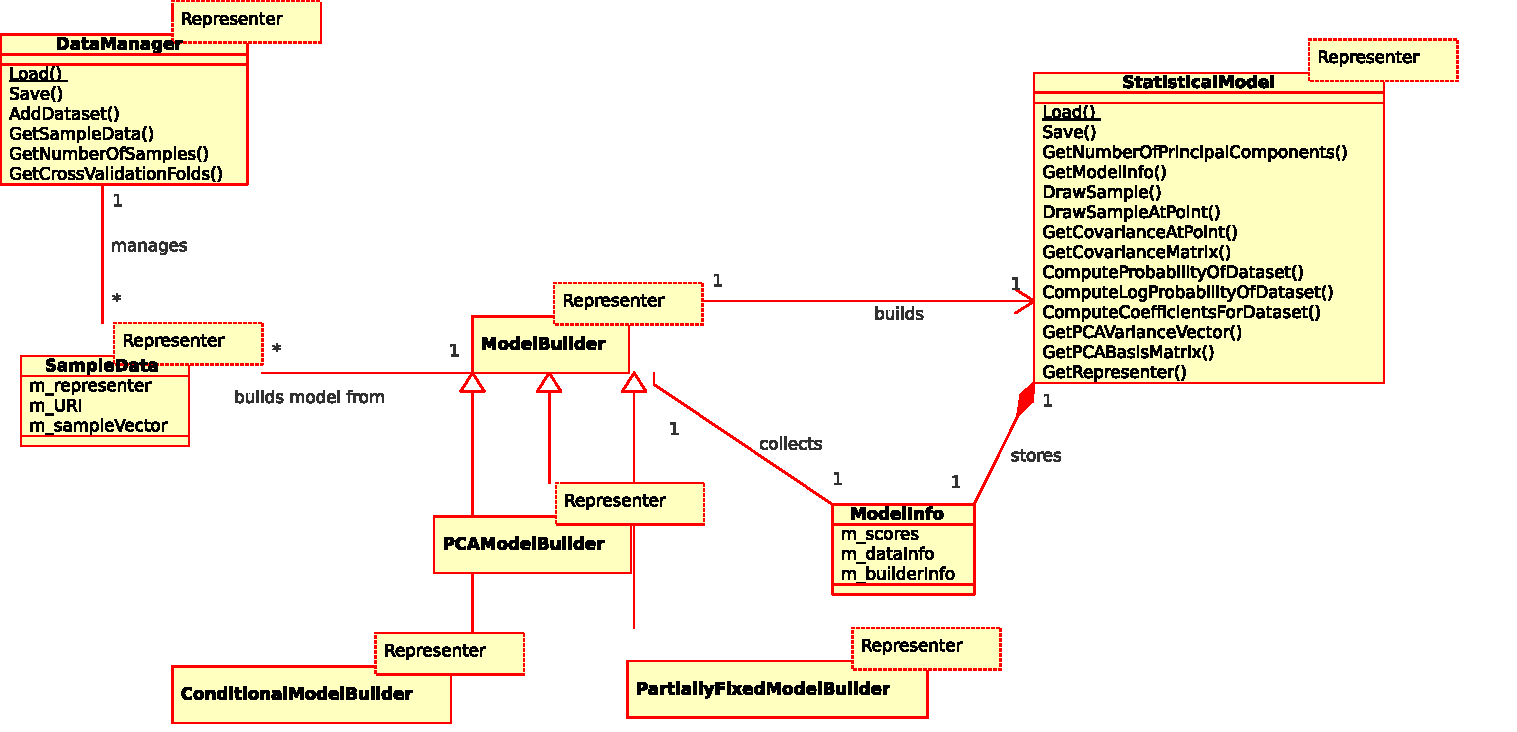
\includegraphics[width=\textwidth]{pictures/class_diagram.pdf}
  \itkcaption{The core classes in \statismo}
  \label{fig:class-diagram}
\end{figure}
All the data used to build the model is added to the data manager
\code{DataManager} class, via the \code{AddDataset} method. This
method converts the dataset into an internal vectorial representation and stores it together
with metadata, such as the URI of the dataset. The \code{ModelBuilder}
class takes a list of these samples and uses it to build a statistical
model. The \code{ModelBuilder} class is also responsible for
collecting all the metadata from the samples, which are then stored
together with additional meta data used by the builder (such as the
build time, parameter settings, etc.) in the \code{ModelInfo}
class. The \code{StatisticalModel} class resulting from the
\code{ModelBuilder} can now be used independently of the other
classes. It contains all the information needed in the application of
the statistical model. We can save the model to a HDF5 file, which can easily be exchanges with 
other researchers. All the information, in particular all the
metadata stored in the \code{ModelInfo}, is contained in the saved file and can
be easily accessed.


We note that most methods defined for the
\code{StatisticalModel} are high level operations, adhering to its
interpretation as a probability distribution. 
These methods all return a valid instance of a dataset modeled by statismo, rather than 
merely its vectorial representation. 
Thus, assuming that statismo is used to build models from \code{itk::Mesh} types, 
the following itk code can be used to 
interact with \statismo:
\begin{verbatim}
itk::Mesh<float, 3>::Pointer mesh = model->DrawSample();
float probability = model->GetProbabilityForDataset(mesh);
\end{verbatim}
This is made possible by the use of so called \code{Representer} classes, over which all the 
classes of \statismo are parametrized.

\subsection{Representers} \label{sec:representers}
The \code{Representer} classes have two distinct purposes:\footnote{
  It could be argued that these two functionalities should be split into two classes. However, this
  makes it much more complicated to ensure the correctness and would lead to even worse error messages
  at compile time.}
First, it is used as an adapter class to convert between the data representation used by the application 
to the internal representation used by \statismo. This allows \statismo to be used with a variety of different toolkits. Second, it also defines how the objects are processed before they are used for building the model.
To  understand the concept behind it, recall from Section~\ref{sec:pca-models}
that before a model is built, an object is discretized, normalized and converted into a vectorial form.
The discretization and normalization step are specific to the type of
object that are modeled.  All classes in \Statismo are parametrized over
a \emph{Representer} class. This representer class provides, among others, the methods
\code{Representer::DatasetToSample}, \code{Representer::SampleToSampleVector} and \code{Representer::SampleVectorToSample}. 
The first method takes care of the discretizaton and normalization, the second method is used to convert a dataset to its vectorial representation. 
The last method is used to convert the vectorial representation back to an object of the modeled type. For a shape model, the first method may for example perform surface registrations on the original meshes,  
followed by a procrustes alignment, the second method transforms the meshes into a vectorial representation, and the last method converts a vector back into a mesh.

\subsection{Special support for ITK}
\Statismo was designed to work together with many different toolkit
and libraries. It was therefore not possible to follow library-specific
conventions. \Statismo has therefore decided to use its own conventions. These
were chosen to make as few assumptions as possible for the user. For example, no smart pointer is used in statismo, as
this would force the user to use the same smart pointer when using
\statismo. As ITK plays such an important role in the community, we
have decided to provide special wrappers that integrate \statismo
directly with ITK and follow the ITK conventions.  This has the
additional advantage that it also becomes possible wrap \statismo
using WrapITK.  The following code snippets illustrate the difference
between the two interfaces:

\begin{verbatim}
statismo::StatisticalModel<RepresenterType>* model = 
    statismo::StatisticalModel<RepresenterType>::Load("model.h5");
SampleType* sample = model->DrawSample();
delete model;
\end{verbatim}
With the itk wrapper, the same code looks like
\begin{verbatim}
itk::StatisticalModel<RepresenterType>::Pointer model = 
    itk::StatisticalModel<RepresenterType>::New();
model->Load("model.h5");
SampleType::Pointer sample = model->DrawSample();
\end{verbatim}
The main difference between the two interfaces, is that the generic \statismo interface 
always provides all the required arguments directly when the object is created
(here with the Load function).
The objects themselves are always well defined after construction and are mostly
immutable.
Furthermore, the generic interface always returns a naked pointer to a newly created object, for which 
the user takes the responsibility to delete. With the ITK Wrapper, all \statismo objects are  ITK objects, and thus 
memory management is automatically done using the \code{itk::SmartPointer}. 

Specifically for ITK, \statismo also provides a class \code{itk::StatisticalModelTransform}, which 
allows us to use statistical models to define an ITK transform, which can be used in the ITK registration 
framework. This allows the user to use all algorithms from this framework for the fitting of statistical models. 


\section{Using \Statismo}
In this section we show how \statismo can be used from applications. We present the first examples using the generic 
interface with the \code{vtkPolyDataRepresenter}. This representer is created by providing it with a reference dataset that 
defines the discretization and mesh topology. Before converting a dataset to its vectorial representation, it performs a Procrustes alignment
\cite{TODO} of the dataset to the reference, and thus normalizes pose variations automatically. Note that this representer assumes, that the datasets are already in correspondence. 

The last example, which illustrates the use of \statismo with the ITK
registration framework, makes use of the ITK Wrappers for statismo. For this we use the \code{itkMeshRepresenter}, which is similar to the \code{vtkPolyDataRepresenter}, but represents
datasets of type \code{itk::Mesh}. Also this representer currently assumes that the meshes are already in correspondence. 


\subsection{Building statistical models in Statismo}

The first step in using \statismo is to define which representer is used and to parametrize all classes with that 
representer. 
\begin{verbatim}
  typedef vtkPolyDataRepresenter RepresenterType;
  typedef PCAModelBuilder<RepresenterType> ModelBuilderType;
  typedef StatisticalModel<RepresenterType> StatisticalModelType;
  typedef DataManager<RepresenterType> DataManagerType;
\end{verbatim}

We create a representer and provide it with a reference. As we are
using the \code{vtkPolyDataRepresenter}, the reference is in this case
a \code{vtkPolyData} object.
Furthermore, we load all the datasets that we wish to use in our model.\footnote{
The \code{loadVTKPolyData} function used in this example is not part of \statismo.}
\begin{verbatim}
  vtkPolyData* reference = loadVTKPolyData("referenceFilename.vtk");
  RepresenterType::Pointer representer = RepresenterType::create(reference);

  vtkPolyData* dataset_1 = loadVTKPolyData(polydataFileName_1);
  ... 
  vtkPolyData* dataset_n = loadVTKPolyData(polydataFileName_n);
\end{verbatim}

These datasets are then added to the \code{DataManager}. Note that we also need to provide the filename as
a second argument to the \code{AddDataset} function. This information will be written as metadata for later
reference. 

\begin{verbatim}
  DataManagerType* dataManager =  DataManagerType::Create(representer);
  dataManager->AddDataset(dataset_1, polydataFileName_1);
  ...
  dataManager->AddDataset(dataset_n, polydataFilename_n);
\end{verbatim}
In the next step we build a model and save it as a HDF5 file. 
\begin{verbatim}
  ModelBuilderType* pcaModelBuilder = ModelBuilderType::Create(representer);
  StatisticalModelType* model =  
      pcaModelBuilder->BuildNewModel(dataManager->GetSampleData(), 0.01);
  model->Save("model.h5");
\end{verbatim}
At the end we need to delete all the create \statismo objects (an alternative would, of course, be to use
smart pointers).
\begin{verbatim}
  delete model;
  delete pcaModelBuilder;
  delete dataManager;
\end{verbatim}

\subsection{Loading a model}
In most applications, the first step is not to build a model, but to load an exisiting model. 
A model is loaded using 
\begin{verbatim}
  typedef vtkPolyDataRepresenter RepresenterType;
  typedef itk::StatisticalModel<RepresenterType> StatisticalModelType;
  StatisticalModelType* model = StatisticalModelType.Load("model.h5");
\end{verbatim}
This restores the full model, including the representer. 
We stress however, that it is important that the same representer is used when loading the model, as the one that was used to build the model. 
\Statismo will throw an exception if this is not the case. 

\subsection{Visualizing the variability}
Probably the first and simplest application that is performed with a new model is to visualize the variability of the modeled objects. 
This can easily be achieved by drawing random samples and visualizing them using standard tools (such as e.g. Paraview). 
\begin{verbatim}
   vtkPolyData* sample = model->DrawSample()
\end{verbatim}
We can also explore the shape space more systematically, by specifying
the PCA coefficients for a given sample. In this example, we obtain three samples:
The mean, a sample corresponding to 3 standard-deviation in the direction of the
first principal component and one corresonding to 3 standard-deviation in the opposite direction.
\begin{verbatim}
   vtkPolyData* mean = model->DrawMean()
   VectorType coeffs = VectorType::Zeros(model->GetNumberOfPrincipalComponents());
   coeffs[0] = 3;
   vtkPolyData* sample1PC1 = model->DrawSample(coeffs);
   coeffs[0] = -3;
   vtkPolyData* sample2PC1 = model->DrawSample(coeffs);
   // ... delete the samples - omitted
\end{verbatim}
Note that each call to DrawSample create a new sample which needs to be deleted by the user.


\subsection{Using statistical models as  a prior}
In many algorithms, statistical models are used as a shape prior. 
A common approach is to take an instance from an algorithm, and project it back into the 
shape space, to get an approximation of the given shape. In statismo, such a projection can be
obtained by computing the PCA coefficients for a given dataset and then restoring it using the 
\code{DrawSample} method:
\begin{verbatim}
vtkPolyData* dataset = someAlgorithm();
VectorType coeffs = model->ComputeCoefficientsForDataset(dataset);
vtkPolyData* projection = model->DrawSample(coeffs);
\end{verbatim}
Often, one simply regularizes an algorithm with the probability. For this purpose, \statismo 
provides a method to compute a (log) probability of a given dataset. 
\begin{verbatim}
float logProbability = model->ComputeLogProbabilityForDataset(aDataset);
\end{verbatim}

\subsection{Cross validation}
An often neglected, but important task is the validation of statistical models. This is usually done by 
checking how well the model can approximate datasets that were not used for model building. 
For this purpose, \statismo provides a cross-validation functionality.

Cross-validation is done using the \code{DataManager}. 
After we have set up the \code{DataManager}, and populated it with the training data, we 
can obtain a list with cross validation folds. 
\begin{verbatim}
typedef DataManagerType::CrossValidationFoldListType CVFoldListType;
CVFoldListType cvFoldList = dataManager->GetCrossValidationFolds(4, true);
\end{verbatim}
Each entry of the \code{cvFoldList} contains a list of training samples and a list with the test samples. 
We iterate over all the folds and build for each fold a new model. A typical validation of the model would 
consist of computing an approximation error between the test sample, and its projection in the model. 
\begin{verbatim}
for (CVFoldListType::const_iterator it = cvFoldList.begin();
     it != cvFoldList.end();
     ++it)
{
    ModelBuilderType* builder = ModelBuilderType::Create();
    StatisticalModelType* model(builder->BuildNewModel(it->GetTrainingData(), 0.01));

    const SampleDataListType testSamplesList = it->GetTestingData();
    for (SampleDataListType::const_iterator it = testSamplesList.begin();
         it != testSamplesList.end()
         ++it)
    {
        vtkPolyData* testSample = (*it)->GetAsNewSample();
        vtkPolyData* projection = model->DrawSample(
                                         model->ComputeCoefficientsForDataset(dataset));
        /// here we could for example compute the approximation error between the 
        /// projection and the test sample - omitted

        testSample->Delete();
    }
    delete modelBuilder;
}

\end{verbatim}

\subsection{Model Fitting using the itk registration framework}\label{sec:model-fitting}
One of the most common applications of statistical models is to fit them to a patient dataset. 
In \Statismo this is done using the ITK registration framework. In the example 
we show how a shape model is fitted to an image using \code{itkPointSetToImageMetric}. 
In this example, we use the ITK wrapper of \statismo, which allow us to use \statismo objects as normal ITK objects.

We start with the usual type definitions. We use for this example a shape model, which has been 
built using the \code{itkMeshRepresenter}. 
\begin{verbatim}
typedef itk::Mesh<float, 3> MeshType;
typedef itk::ImageType<float, 3> ImageType
typedef itk::MeshRepresenter<float, 3> RepresenterType;
typedef itk::StatisticalShapeModelTransform<RepresenterType, double, 3> TransformType;
typedef itk::MeanSquaresPointSetToImageMetric<MeshType, ImageType> MetricType;
\end{verbatim}
The StatisticalShapeModelTransform is a class defined by \statismo. It is a subclass of the \code{itk::Transform}
and can thus be directly used wherever an \code{itk::Transform} is expected. 

In the next step we load the model and obtain the reference mesh that was used to build the model via
the representer. This mesh is used by the \code{PointSetToImageMetric}, and determines the points on which the 
metric is evaluated. 
\begin{verbatim}
StatisticalModelType::Pointer model = StatisticalModelType::New();
model->Load(modelname);
MeshType::Pointer fixedPointSet  = model->GetRepresenter()->GetReference();
\end{verbatim}

The transform is set up by setting the statistical model, and initializing it to the identity transform. 
\begin{verbatim}
TransformType::Pointer transform = TransformType::New();
transform->SetStatisticalModel(model);
transform->SetIdentity();
\end{verbatim}

The registration is then set up in the usual way. We omit here the details.
\begin{verbatim}
MetricType::Pointer metric = MetricType::New()
...

RegistrationFilterType::Pointer registration = RegistrationFilterType::New();
registration->SetInitialTransformParameters(transform->GetParameters());
registration->SetTransform(   transform );
registration->SetFixedPointSet( fixedPointSet );
...
registration->Update()
\end{verbatim}

After a successful registration, the transform parameters correspond to the PCA coefficients in our model. 
To obtain the final mesh, we can obtain these coefficients from the transform using the method \code{GetCoefficients} 
and draw the corresponding sample from the model. 
\begin{verbatim}
MeshType::Pointer finalMesh = model->DrawSample(transform->GetCoefficients());
\end{verbatim}


\section{Adding more prior information: Constrained PCA models }
One goal of \statismo is to allow the integration of  different algorithms for building statistical models.
Currently, \statismo comes with three different methods to build statistical models (Cf. Figure~\ref{fig:class-diagram}). Besides the standard \code{PCAModelBuidler} that was used in all the examples presented so far, there is a \code{PartiallyFixedModelBuilder} \cite{TODO} and a \code{ConditionalModelBuilder} \cite{TODO}. Both model builders incorporate additional prior information into the model building and thus reduce the variability of the resulting model. The resulting models itself, are standard PCA models that can be used and interpreted in exactly the same way as the models discussed so far. 

\subsection{Partially fixed models}
\begin{figure}
  to be included
  \itkcaption{A constrained model (TODO text)}
    \label{fig:constrained-model}
\end{figure}
Partially fixed models allow for introducing geometric constraints on the model. For example, a part of the shape may be known, and only the flexibility of the remaining part should be obtained. Another typical scenario is when in an application of the shape model, the user provides a number of landmarks that fix the shape. 
Consider the shape model fitting example from Section~\ref{sec:model-fitting}. Assume that we have a set of landmark points, which determine the position of the target shape. We can incorporate these points already into the model building, to obtain a model that is fixed at the landmark points. Figure~\ref{fig:constrained-model} shows an example of such a  constrained model.  Using this model for model fitting leads to a simpler optimization problem, and furthermore guarantees that the landmark points are matched. 
The following (incomplete) code illustrates how such models can be built. 

\begin{verbatim}
// ... usual type definitions - omitted
typedef PartiallyFixedModelBuilder<RepresenterType> PartiallyFixedModelBuilderType;

PartiallyFixedModelBuilderType*  pfmb = PartiallyFixedModelBuilderType::Create();

// ... Read source and target landmarks, omitted

StatisticalModelType::PointValueListType constraints;
for (unsigned i = 0; i < numLandmarks; i++) { 
   StatisticalModelType::PointValuePairType cnstr(sourceLandmarks[i] , targetLandmarks[i]);
   constraints.push_back(cnstr);
}
StatisticalModelType* constraintModel = 
   pfmb->BuildNewModel(dataManager->GetSampleData(), constraints);
\end{verbatim}

For more details about the idea of these models, we refer to the papers \cite{Mathsurface, PriorDeformation}.

\subsection{Conditional Models}
The second algorithm for building , which we refer to asthe \emph{ConditionalModelBuilder} for constrained model is used when there are additional surrogate information about the data available. For example (TODO REMI, can you write a good introduction here)
We refer to \cite{TODO cite remi's paper}. 

\section{Conclusion}
In this paper we have presented \statismo, which is a framework for
PCA based statistical models.  \Statismo implements a high level view
on PCA models by interpreting these models as normal distribution over
the modeled objects. The underlying low level vectorial representation
of the object is never exposed to the user.  The conversion between
the data representation by the user, and the vectorial representation
used by \statismo is done by special Representer classes, which are
defined for each data representation. This allows \statismo to ensure
that the same discretization and normalization steps are applied when
using the model, as those that were used during model building.  A
statistical model in \statismo thus always have a well defined
interpretation and semantics.  This, together with the fact that
\statismo writes all its information into a single, portable HDF5
file, makes the exchange of statistical models built with \statismo
easy. To use the model, the user only needs to have access to the same Representer that was used to build the model. 

\Statismo comes with ready made Representer classes for the most important object representations used in VTK and ITK. 
Currently all these representers require that the data is already in correspondence. It is, however, easily possible to 
write representers that also establish correspondence, and thus to cover the full model creation pipeline with \statismo.
By writing custom representers, it becomes also possible to use \statismo with other toolkits than ITK or VTK. 

Statismo also makes it easy to integrate new methods for building models. Our hope is, that the number of different representers
and model builders will grow and thus \statismo will become a more and more powerful toolkit for building a large variety of differnet 
models.




\appendix

\section{Appendix}
\subsection{A list of standard representers}\label{app:representers}
TODO to be rewritten

The following representers are shipped with \statismo:

\begin{tabular}{ll}
  Name & Description \\ \hline 
  vtkPolyDataRepresenter & Shape models from vtk meshes.  \\
  & The examples are aligned to a reference using Procrustes alignment \\
  & No registration is performed - Examples have to be in correspondence. \\ \\
  vtkStructuredPointsRepresenter & Image models and Deformation models from vtk structured points.\\
  & No registration is performed - Examples have to be in correspondence. \\ \\
  itkImageRepresenter & Image (intensity) models from itk images \\
  & No registration is performed - Examples have to be in correspondence. \\ \\
  itkVectorImageRepresenter & Deformation models from itk displacement fields. \\
  & No registration is performed - Examples have to be in correspondence. \\ \\
  itkVectorLMAlignImageRepresenter & Deformation models from itk displacement fields \\
  & All deformation fields are aligned rigidly to a number of specified points. \\
  & No registration is performed - Examples have to be in correspondence. \\ \\

\end{tabular}
\subsection{Defining your own representer}
TODO to be rewritten
Consider the method
\code{ComputeProbabilityForDataset(DatasetConstPointType object)} defined for the \code{StatisticalModel}. This probability 
can only be computed in a meaningful way if the object is discretized and normalized exactly in the same way 
as it was done for the training data. Therefore, a model is only well defined if it is used with the same \code{Representer} as was used to create the model.

For specifying the semantics, a \code{Representer} implements the following methods:
\begin{verbatim}
	DatasetPointerType DatasetToSample(DatasetConstPointerType ds) const;
	VectorType SampleToSampleVector(DatasetConstPointerType sample) const;
	DatasetPointerType SampleVectorToSample(const VectorType& sample) const;
	statismo::VectorType PointSampleVectorToPointSample(const ValueType& v) const;
	ValueType PointSampleToPointSampleVector(const VectorType& pointSample) const;
\end{verbatim}
The terminology used in this definitions is the following: 
\begin{description}
  \item[Dataset] A dataset is a representation of an object in the specific toolkit, such as e.g. a vtkPolyData or a itk::Mesh
  \item[Sample] A sample is of the same type as the Dataset, but is discretized and normalized as discussed in Section~\ref{sec:pca-models}. 
  \item[SampleVector] The SampleVector denotes the vectorial representation of a sample.
  \item[PointSample] This refers to the value of a sample at a given point. For an mesh this would for example be a point of the mesh, for a  image, this would denote a pixel value (e.g. image intensity).
  \end{description}
  
  Defining these methods allows for a great variety of different models. On one
  hand, one could imagine implementing a representer that covers the whole
  pipeline including discretization and registration. At the other extreme, a representer may simply take vectorized data directly, without specifying any registration or normalization strategy.

To make the use of \statismo easier for the user, \Statismo already provides a number of representers for the most common applications. See \ref{app:representers} for a list of predefined representers. 

\subsection{The file format}
TODO to be rewritten
The statistical models are stored in a HDF5 file format (TODO cite). HDF5 was chosen, as it allows for the efficient and platform independent storage of large data. HDF5 provides a hierarchical organization to store the data, similar to what is known from the common file systems. For \statismo, we have defined 3 main groups:
\begin{description}
  \item [model] Contains the vectors matrices that make up the model. This information is stored under the keys \code{mean}, \code{pcaBasis}, \code{pcaVariance} and \code{noiseVariance}. 
  \item [modelinfo] Contains all the metadata for this model. The metadata consists of the \code{scores} (the PCA coefficients of the original example data), a section \code{builderInfo} containing all the parameters from the model builders, as well as a section \code{dataInfo} containing information about the data used to build this model, such as the URI's of the original examples. 
  \item [representer]
    This group is used to store all the information that is needed by a specific representer. 
\end{description}

\section{TODO}
\begin{itemize}
  \item include examples
  \item mention VSD
\end{itemize}

\subsection*{Acknowledgements}
This work has been supported by the CO-ME/NCCR research network of
the Swiss National Science Foundation. We thank Arnauld Gelas for helpful comments regarding this
submission. 

%%%%%%%%%%%%%%%%%%%%%%%%%%%%%%%%%%%%%%%%%%%%%%%%%%%%%%%%%%
%
%  Example on how to insert a figure
%
%%%%%%%%%%%%%%%%%%%%%%%%%%%%%%%%%%%%%%%%%%%%%%%%%%%%%%%%%%

%\begin{figure}
%\center
%\includegraphics[width=0.8\textwidth]{RegistrationComponentsDiagram.eps}
%\itkcaption[Registration Framework Components]{The basic components of the
%registration framework are two input images, a transform, a metric, an
%interpolator and an optimizer.}
%\label{fig:RegistrationComponents}
%\end{figure}





%%%%%%%%%%%%%%%%%%%%%%%%%%%%%%%%%%%%%%%%%
%
%  Insert the bibliography using BibTeX
%
%%%%%%%%%%%%%%%%%%%%%%%%%%%%%%%%%%%%%%%%%

\bibliographystyle{plain}
\bibliography{InsightJournal}


\end{document}

